\documentclass[12pt]{article}
\usepackage{amssymb, amsmath}
\usepackage{fancyhdr,lastpage}
\usepackage{amsmath,amsfonts,amssymb}
\usepackage{graphicx}
\usepackage{stix}
\usepackage{enumitem}
\usepackage{listings}
\tolerance 10000
\headheight 0in
\headsep 0in
\evensidemargin 0in
\oddsidemargin \evensidemargin
\textwidth 6.5in
\topmargin .25in
\textheight 8.7in

\newcommand{\CC}{{\mathbb C}}
\newcommand{\QQ}{{\mathbb Q}}
\newcommand{\RR}{{\mathbb R}}
\newcommand{\ZZ}{{\mathbb Z}}
\newcommand{\NN}{{\mathbb N}}
\newcommand{\FF}{{\mathbb F}}


\newcommand{\Zerobold}{{\boldsymbol 0}}
\newcommand{\Onebold}{{\boldsymbol 1}}
\newcommand{\xbold}{{\boldsymbol x}}

\newcommand{\mfrak}{{\mathfrak m}}

\newcommand{\Acal}{{\mathcal A}}
\newcommand{\Ncal}{{\mathcal N}}
\newcommand{\Pcal}{{\mathcal P}}
\newcommand{\Qcal}{{\mathcal Q}}

\newcommand{\sqbinom}[2]{\genfrac{[}{]}{0pt}{}{#1}{#2}}
\newcommand{\angbinom}[2]{\genfrac{\langle}{\rangle}{0pt}{}{#1}{#2}}

\newcommand{\qddx}{(d/dx)_{q}}

%\newcommand{\pfcl}{\emph{Proof of claim}}
\newenvironment{proof}{\paragraph{Proof: }}{\hfill$\blacksquare$}



\def\multiset#1#2{\ensuremath{\left(\kern-.3em\left(\genfrac{}{}{0pt}{}{#1}{#2}\right)\kern-.3em\right)}}


\DeclareMathOperator{\des}{des}
\DeclareMathOperator{\maj}{maj}
\DeclareMathOperator{\ev}{ev}
\DeclareMathOperator{\Hom}{Hom}
\DeclareMathOperator{\trace}{tr}
\DeclareMathOperator{\inv}{inv}

\newtheorem{problem}{Problem}%[section]

\begin{document}

\begin{center}
{\bf Julio Soldevilla}
\\
{\bf EECS 545 Winter 2018 --- Problem Set 2 }
\end{center}

\begin{problem}
\normalfont
Problem 1
\end{problem}

\begin{proof}
\begin{enumerate}
\item For the first part of this problem, for the linear regression we get a test error of $0.4996621$ and we get a the following plot predicting the labels for the test instances:

\begin{figure}[!htbp]
\centering
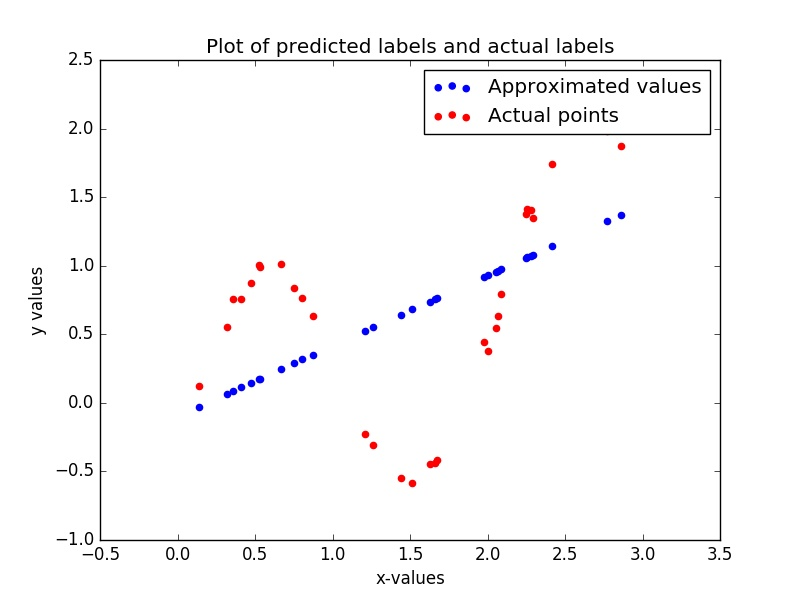
\includegraphics[width=10cm]{hw2_p1_linreg.jpg}
\caption{Image showing the plot of the prediction using linear regression}
\end{figure}


\item For the second part of this problem, we use locally weighted linear regression. In this part of the problem, we found that when $\tau = 0.2$, we get a test error of $0.01395202$ and when $\tau = 2$, we get a test error of $0.4253173$. Also, we present plots showing the prediction lables with the actual labels for the test instances when $\tau = 0.2$ (first figure below) and when $\tau = 2$ (second figure below).

\begin{figure}[!htbp]
\centering
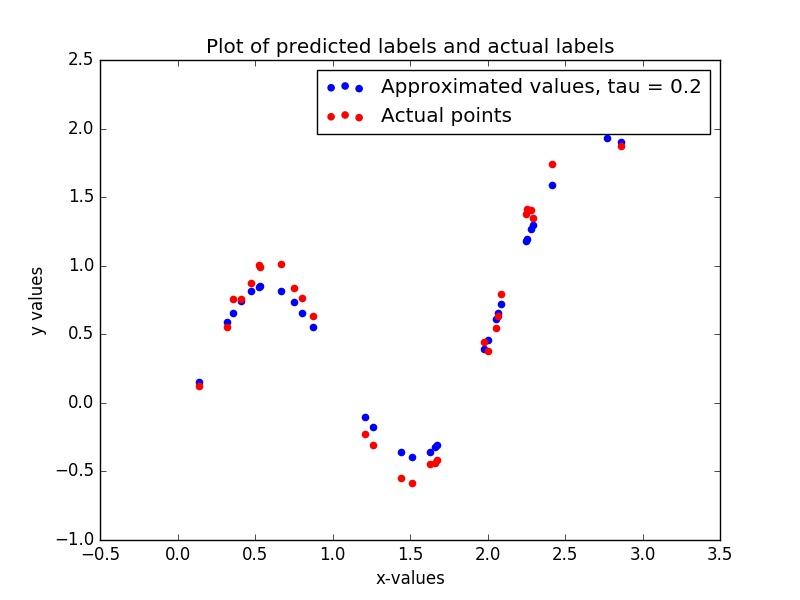
\includegraphics[width=10cm]{hw2_p1_loc_weight_t1.jpg}
\caption{\textbf{Problem 1b:} Image showing the plot of the prediction using locally weighted linear regression and $\tau = 0.2$}
\end{figure}

\begin{figure}[!htbp]
\centering
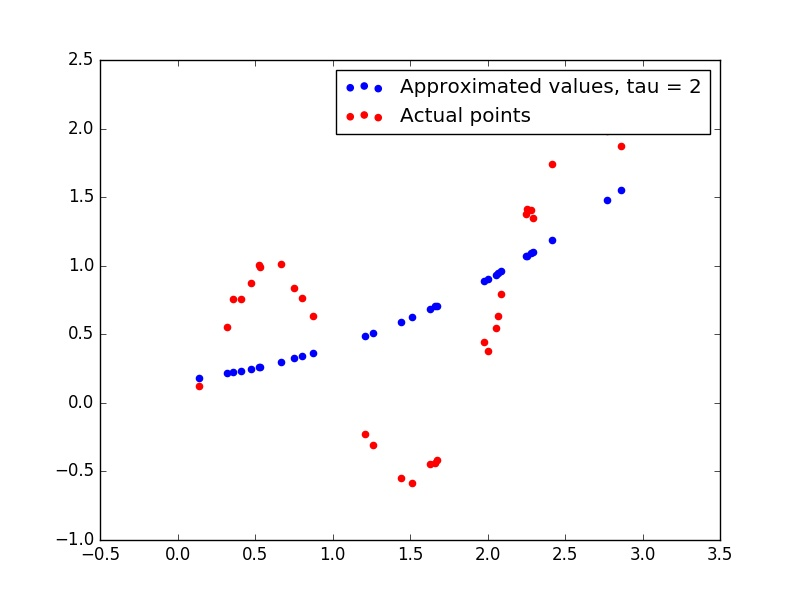
\includegraphics[width=10cm]{hw2_p1_loc_weight_t2.jpg}
\caption{\textbf{Problem 1b:} Image showing the plot of the prediction using locally weighted linear regression and $\tau = 2$}
\end{figure}

\end{enumerate}
\end{proof}

\begin{problem}
\normalfont
Problem 2
\end{problem}

\begin{proof}
\begin{enumerate}
\item This part of the problem is in the code submitted to canvas.

\item In this part of the problem, we found that the marginal distribution $P(X_1)$ is a normal distribution with mean $\mu = 0$ and standard deviation $\sigma = 1$. The plot of this distribution is the following one:

\begin{figure}[!htbp]
\centering
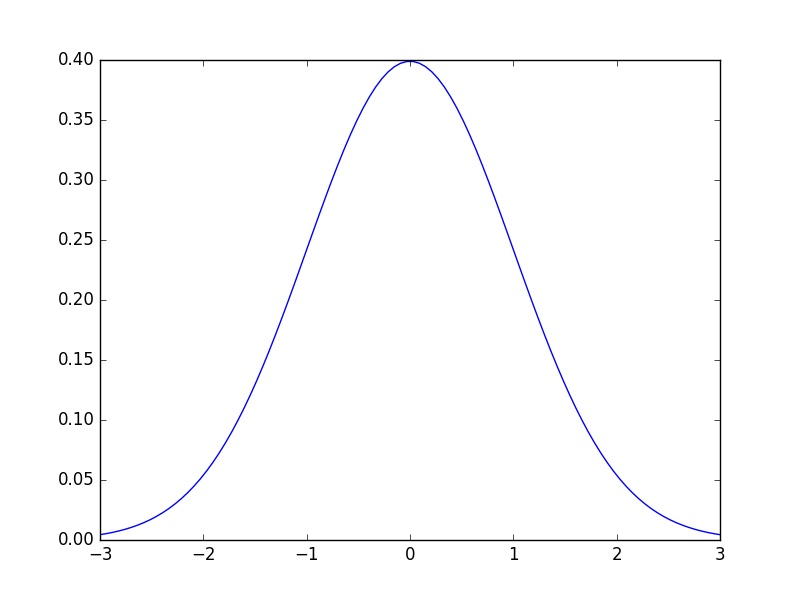
\includegraphics[width=10cm]{hw_p2_marginal_distribution.jpg}
\caption{\textbf{Problem 2a:} Image showing hte marginal distribution $P(X_1)$}
\end{figure}

\item The solution of this problem is in the code submitted to canvas.

\item In this part of the problem, we found that the marginal distribution $P(X_1,X_4|X_2 = 0.1,X_3 = -0.2)$ follows a normal distribution with mean $\mu = \left[ \begin{matrix} 0.55 & 0.15 \end{matrix}\right]$ and covariance matrix $\Sigma = \left[ \begin{matrix}0.75 & -0.75 \\ -0.75 & 1.75 \end{matrix}\right]$. The heat map of this distribution is shown below:

\begin{figure}[!htbp]
\centering
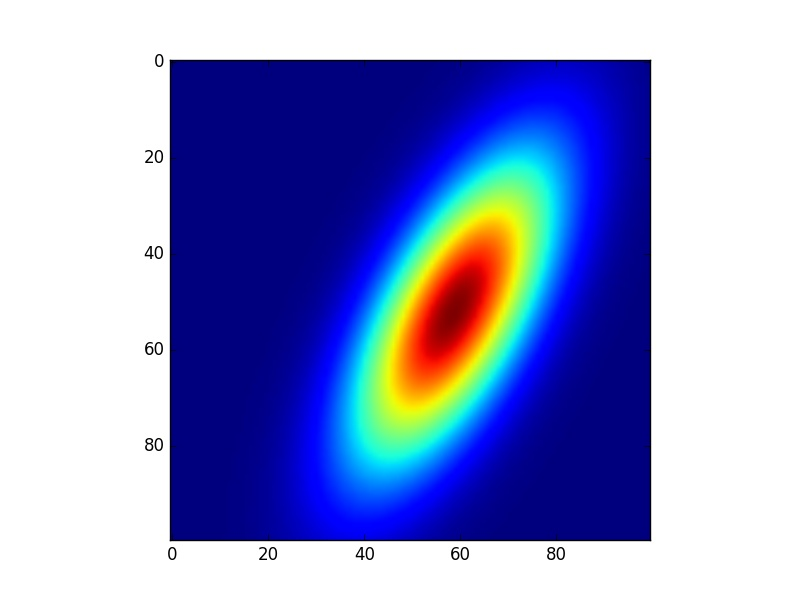
\includegraphics[width=10cm]{hw2_p2_conditional.jpg}
\caption{\textbf{Problem 2b:} Image showing the conditional distribution $P(X_1,X_4|X_2 = 0.1,X_3 = -0.2)$}
\end{figure}

\end{enumerate}
\end{proof}

\begin{problem}
\normalfont
Problem 3
\end{problem}

\begin{proof}
Our solution for this problem is presented in the following list, which presents the mean and covariance matrices for a particular instance:

\begin{enumerate}
\item This is the mean for initial distribution of w $\left[\begin{matrix} 0.31207185 & -0.38444814\end{matrix}\right]$
This is the covariance matrix for initial distribution of w $\left[ \begin{matrix} 0.40995687 & 0.1109261 \\  0.1109261  & 0.36334771 \end{matrix} \right]$

\item This is the mean for the distribution of w after 1 instance(s) $\left[\begin{matrix}  0.31207185 & -0.38444814\end{matrix}\right]$
This is the covariance matrix for the distribution of w after 1 instance(s) $\left[ \begin{matrix} 0.40995687 & 0.1109261 \\ 0.1109261  & 0.36334771\end{matrix} \right]$

\item This is the mean for the distribution of w after 10 instance(s) $\left[\begin{matrix}  0.97746676& -0.52199623\end{matrix}\right]$
This is the covariance matrix for the distribution of w after 10 instance(s) $\left[ \begin{matrix}  0.06639281 & -0.02378635 \\ -0.02378635 & 0.0918552  \end{matrix} \right]$

\item This is the mean for the distribution of w after 20 instance(s) $\left[\begin{matrix}  0.43026927 &-0.22064332\end{matrix}\right]$
This is the covariance matrix for the distribution of w after 20 instance(s) $\left[ \begin{matrix}  0.01792457 & -0.00630496 \\ -0.00630496 & 0.04767232 \end{matrix} \right]$

\end{enumerate}

The plots for each of the four cases above are presented below:

\begin{figure}[!htbp]
\centering
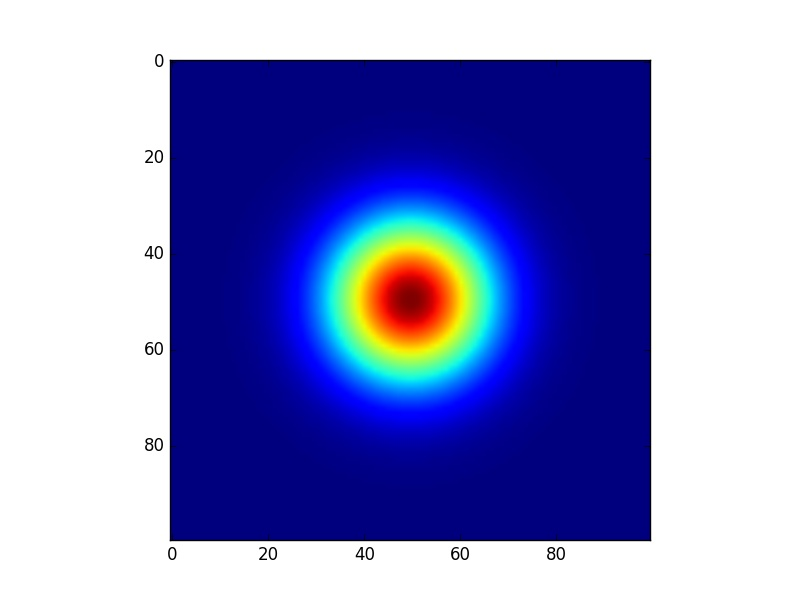
\includegraphics[width=8cm]{hw2_p3_w_initial.jpg}
\caption{\textbf{Problem 3:} Image showing the initial distribution of $w$}
\end{figure}

\begin{figure}[!htbp]
\centering
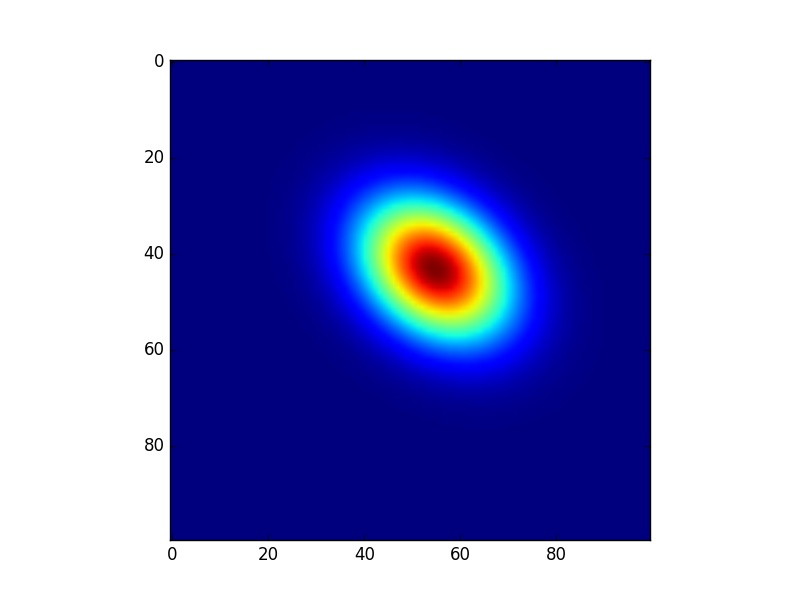
\includegraphics[width=8cm]{hw2_p3_w_1.jpg}
\caption{\textbf{Problem 3:} Image showing the distribution of $w$ after 1 instance}
\end{figure}

\begin{figure}[!htbp]
\centering
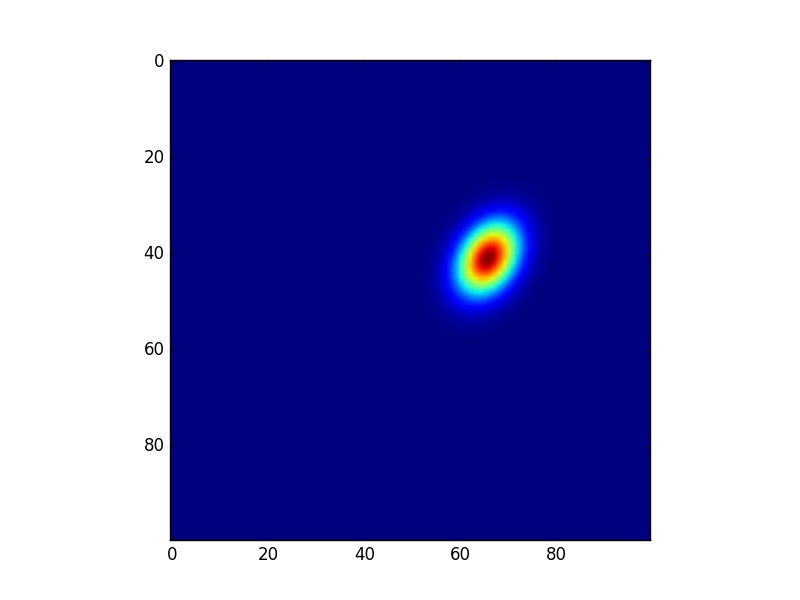
\includegraphics[width=8cm]{hw2_p3_w_10.jpg}
\caption{\textbf{Problem 3:} Image showing the distribution of $w$ after 10 instance}
\end{figure}

\begin{figure}[!htbp]
\centering
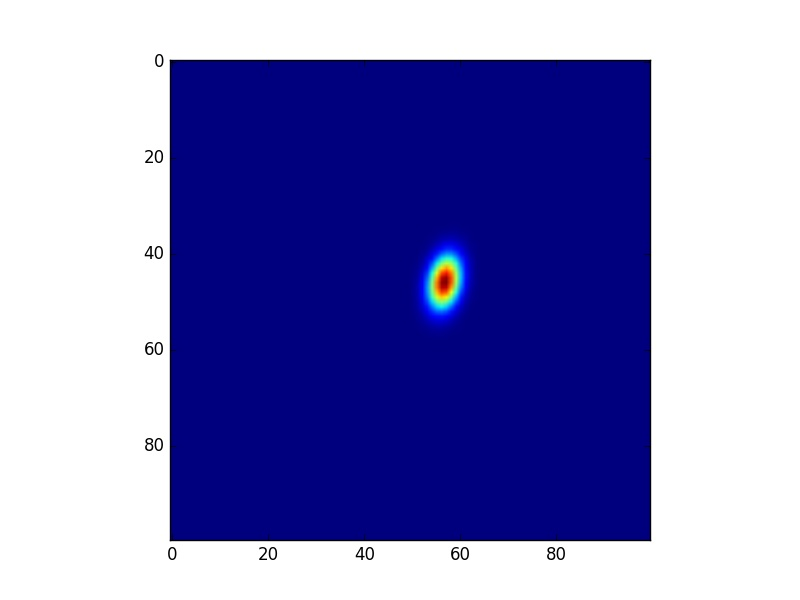
\includegraphics[width=8cm]{hw2_p3_w_20.jpg}
\caption{\textbf{Problem 3:} Image showing the distribution of $w$ after 20 instances}
\end{figure}

\end{proof}

\begin{problem}
\normalfont
Problem 4
\end{problem}

\begin{proof}
\begin{enumerate}
\item Part a is divide into two smaller parts
	\begin{enumerate}
		\item The joint distribution over $y(x_1),...,y(x_n)$ is Gaussian distribution, with mean $\mu = \vec{0}$ where $\mu$ has size $n \times 1$ and covariance matrix $\Sigma_{n} = \left[ \begin{matrix} exp^{-\frac{\|x_1 - x_1\|^2}{2 \sigma^2}} & exp^{-\frac{\|x_1 - x_2\|^2}{2 \sigma^2}} & \dots & exp^{-\frac{\|x_1 - x_n\|^2}{2 \sigma^2}} \\ exp^{-\frac{\|x_2 - x_1\|^2}{2 \sigma^2}} & exp^{-\frac{\|x_2 - x_2\|^2}{2 \sigma^2}} & \dots & exp^{-\frac{\|x_2 - x_n\|^2}{2 \sigma^2}} \\ \vdots & \dots & \dots & \vdots \\ exp^{-\frac{\|x_n - x_1\|^2}{2 \sigma^2}} & exp^{-\frac{\|x_n - x_2\|^2}{2 \sigma^2}} & \dots & exp^{-\frac{\|x_n - x_n\|^n}{2 \sigma^2}} \end{matrix}\right]$
		\item The following figures are the plots for the  sampling form the GP prior shown above. Each figure corresponds to one value of $\sigma = \{0.3,0.5,1\}$

		\begin{figure}[!htbp]
\centering
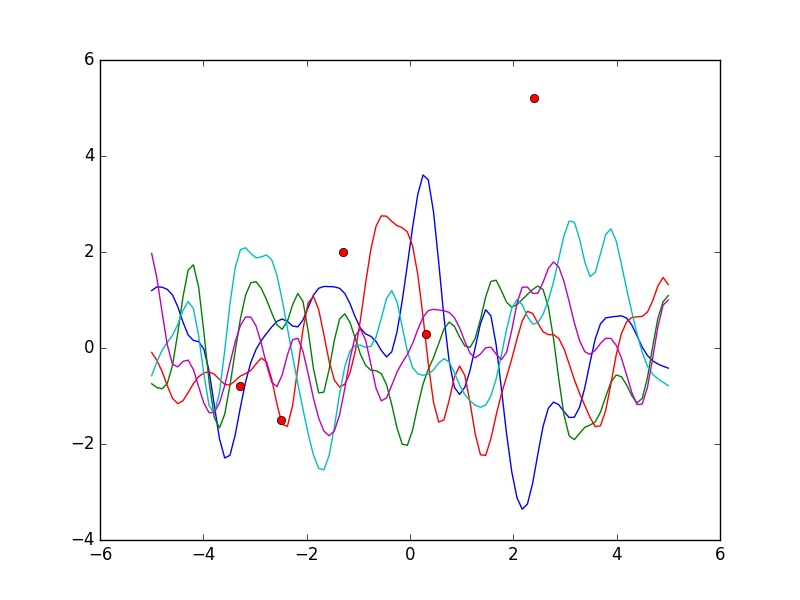
\includegraphics[width=8cm]{hw_p4_prior_03.jpg}
\caption{\textbf{Problem 4:} Image showing the  5 samples from the GP with $\sigma = 0.3$}
\end{figure}

		\begin{figure}[!htbp]
\centering
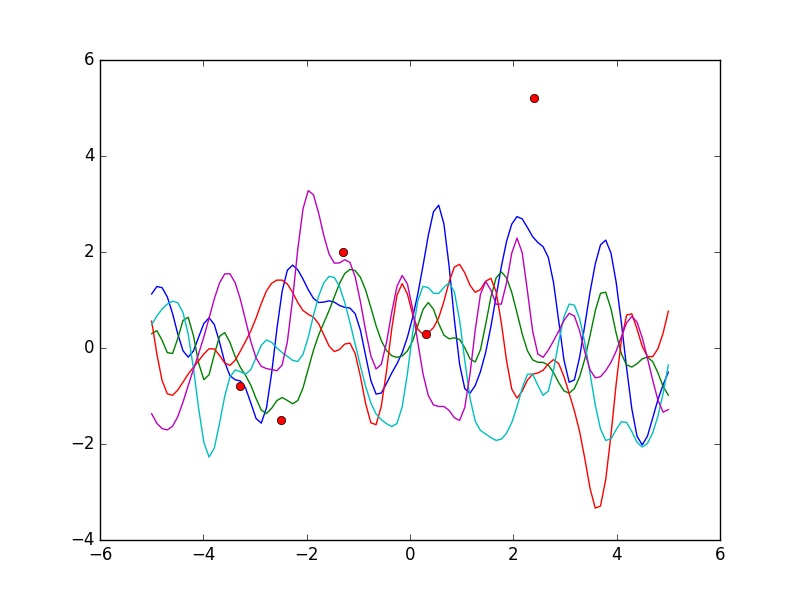
\includegraphics[width=8cm]{hw_p4_prior_05.jpg}
\caption{\textbf{Problem 4:} Image showing the  5 samples from the GP with $\sigma = 0.5$}
\end{figure}

		\begin{figure}[!htbp]
\centering
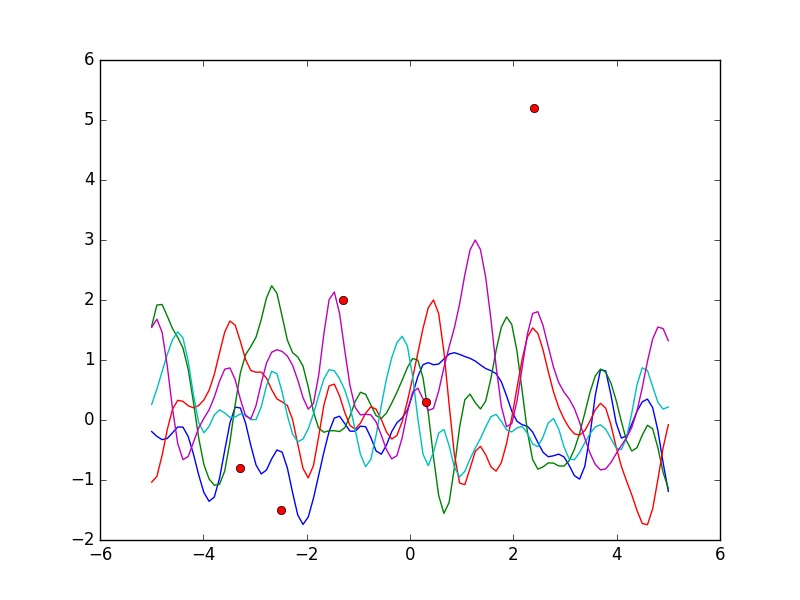
\includegraphics[width=8cm]{hw_p4_prior_1.jpg}
\caption{\textbf{Problem 4:} Image showing the  5 samples from the GP with $\sigma = 1$}
\end{figure}


	\end{enumerate}

\item Part b is also divided in 2 parts:

\begin{enumerate}
		\item This time, again the posterior follows a Gaussian distribution, with similar mean and sigma as above. 
		\item The following figures are the plots for the  sampling form the GP posterior shown above. Each figure corresponds to one value of $\sigma = \{0.3,0.5,1\}$

		\begin{figure}[!htbp]
\centering
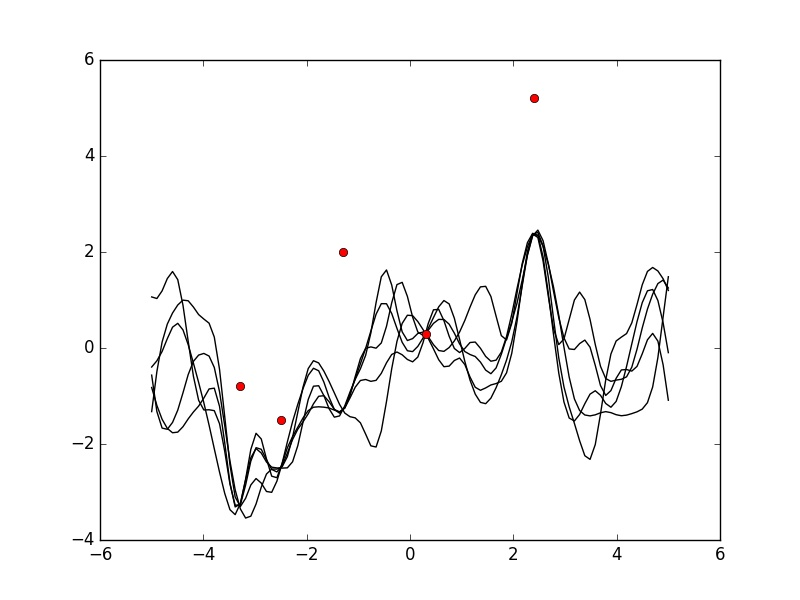
\includegraphics[width=8cm]{hw_p4_03.jpg}
\caption{\textbf{Problem 4:} Image showing the  5 samples from the posterior GP with $\sigma = 0.3$}
\end{figure}

		\begin{figure}[!htbp]
\centering
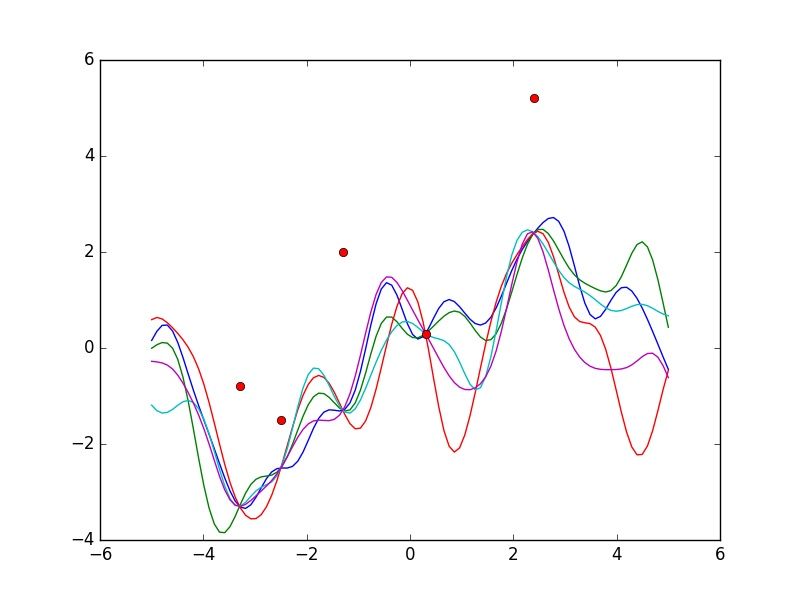
\includegraphics[width=8cm]{hw_p4_05.jpg}
\caption{\textbf{Problem 4:} Image showing the  5 samples from the posterior GP with $\sigma = 0.5$}
\end{figure}

		\begin{figure}[!htbp]
\centering
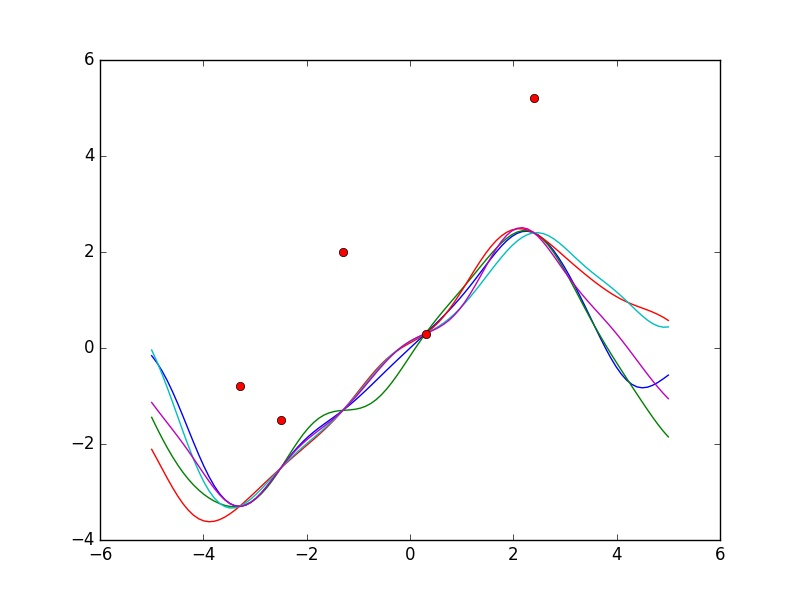
\includegraphics[width=8cm]{hw_p4_1.jpg}
\caption{\textbf{Problem 4:} Image showing the  5 samples from the posterior GP with $\sigma = 1$}
\end{figure}
\end{enumerate}

\end{enumerate}
\end{proof}

\begin{problem}
\normalfont
Problem 5
\end{problem}

\begin{proof}
For this problem, for \textbf{part a)}, we present a plot that shows the linear hyperplane dividing the points we found using only the perceptron update rule. This is the shown in the followin picture.

\begin{figure}[!htbp]
\centering
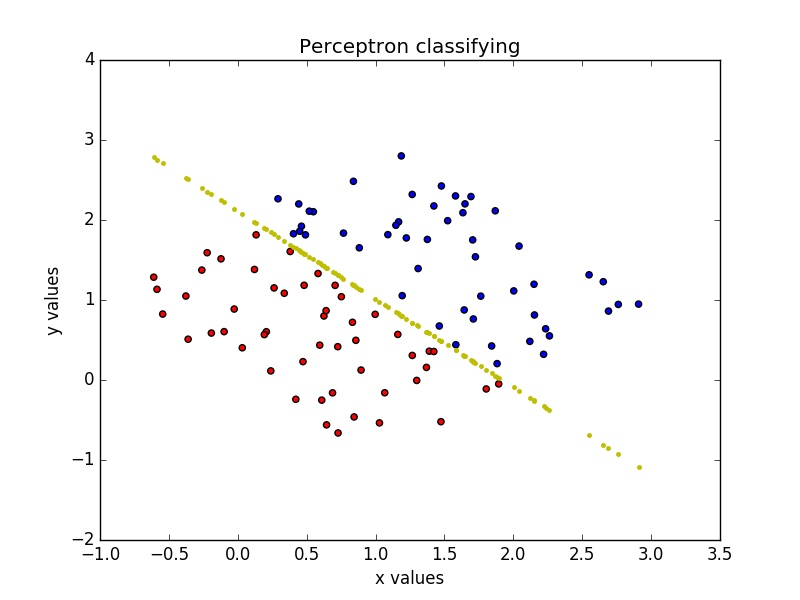
\includegraphics[width=8cm]{hw2_p5_perceptron.jpg}
\caption{\textbf{Problem 5:} Image showing the linear hyperplane dividing the points found usng only the perceptron update rule}
\end{figure}

For \textbf{part b)} of the problem, we do the same analysis for a set of data that doesn't have a linear separation. IN this case, we present the linear separation found by the perceptron update algorithm plotted with yellow points in the figure below. We can see that this line is not as good as it can be. To improve we apply also the pocket algorithm, which implies that we will store in memory the vector of $w$ that produces the highest correct predictions throughout the algorithm. If the vector $w$ that the algorithms ends with has a higher matching rate, then we use an output of the algorithm the last $w$. If the vector $w$ we were saving throughout the algorithm is better, then we take as an output the saved vector $w$. In this way, we make sure we have the vector of coefficient that produces the most matches. In the figure below, the line in black is obtained using the vector $w$ from the pocket algorithm and we can see that it does a better job of classifying the points.

\begin{figure}[!htbp]
\centering
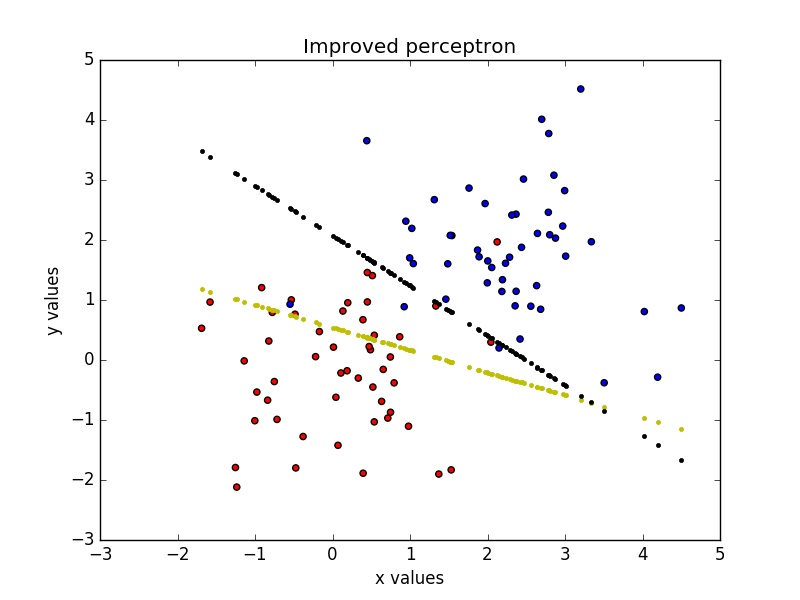
\includegraphics[width=10cm]{hw2_p5b_perceptron_update.jpg}
\caption{\textbf{Problem 3:} Image showing linear hyperplane dividing the points found using only the perceptron update rule and the pocket algorithm. The yellow line is obtained using only the perceptron update rule and the other black line is obtained using the pocket algorithm}
\end{figure}

\end{proof}

\begin{problem}
\normalfont
Problem 6
\end{problem}

\begin{proof}
For this problem we found that the weight vector without bias term is: $[ 0.49230156, -1.02181685, -0.38697494, -0.70922472, -0.02087894,  0.14882702,
 -0.07118593, $ $-0.09869681,  0.15392742,  0.58795622, -0.05514312,  0.82930682,
 -0.62670417,  0.32124253, -0.79053791,$ $ 0.55524013, -0.44701531, -0.75471243,
 -0.26418911, -0.21516875, -0.9294681,   0.03643845, $ $-0.11790563, -0.26960344,
 -0.42819214,  0.35976133, -0.90088309, -1.05377673,$ $ -0.54921289,  0.60597135]$

Also, for this problem, this is the final training cross entropy: $0.193449363355$, this is the final test cross entropy: $0.181117073447$, this is the final training classification accuracy percentage: $93.43832021\% $ and this is the final test classification accuracy percentage: $94.1489361702 \%$

Finally, the plots for the training and test classification accuracy vs number of iterations (first picture) and the plot of average training and test erros vs number of iterations (second picture) are shown below. 

\begin{figure}[!htbp]
\centering
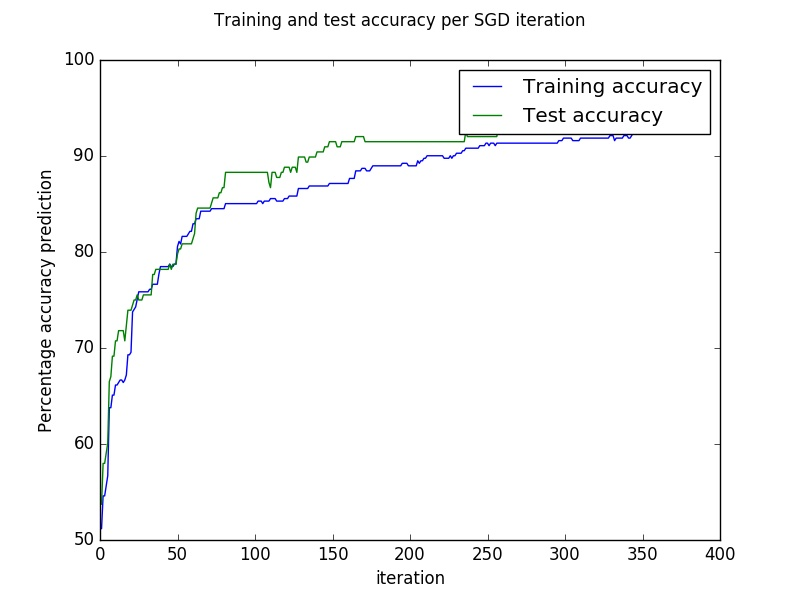
\includegraphics[width=10cm]{hw2_p6_accuracy.jpg}
\caption{\textbf{Problem 6}: Image showing the training and test classification accuracy vs number of iterations plot}
\end{figure}

\begin{figure}[!htbp]
\centering
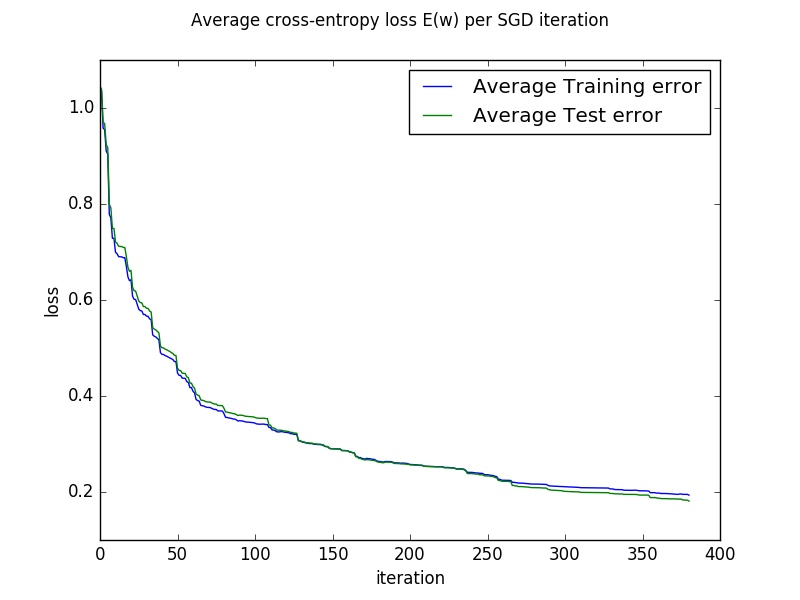
\includegraphics[width=10cm]{hw2_p6_cross_entropy.jpg}
\caption{\textbf{Problem 6}: Image showing the training and test cross entropy vs number of iterations plot}
\end{figure}

\end{proof}
\end{document}